\documentclass[twoside,twocolumn]{article}
\usepackage{charter}
\usepackage[T1]{fontenc}
\usepackage[english]{babel}
\usepackage[hmarginratio=1:1,top=32mm,columnsep=20pt,margin=1.15in]{geometry}
\usepackage{graphicx}
\usepackage{abstract}
\renewcommand{\abstractnamefont}{\normalfont\large\scshape\bfseries}
\renewcommand{\abstracttextfont}{\normalfont\normalsize\itshape}

\usepackage{titlesec}
\renewcommand\thesection{\Roman{section}}
\titleformat{\section}[block]{\large\scshape\bfseries\centering}{\thesection.}{1em}{}
\renewcommand\thesubsection{\roman{subsection}}
\titleformat{\subsection}[block]{\normalsize\itshape\bfseries}{\thesubsection.}{1em}{}

\usepackage{titling}
\usepackage{hyperref}
\newcommand\tab[1][1cm]{\hspace*{#1}}




\usepackage[symbol]{footmisc}

\renewcommand{\thefootnote}{\fnsymbol{footnote}}






\pretitle{
    \begin{center}
    \Huge
}

\posttitle{
    \end{center}
    \begin{center}
        \textit{
            \large A cryptographically secure online voting portal for small scale elections.
        }
    \end{center}
}

\title{
    \textbf{Online Election Manager}
}

\author{
    \\
    \\
    \textbf{\textsc{Priydarshi Singh}}\\
    \normalsize First Year Undergraduate \\
    \normalsize Department of Aerospace Engineering \\
    \normalsize Indian Institute Of Technology, Kanpur \\
    \normalsize \href{mailto:darshi@iitk.ac.in}{darshi@iitk.ac.in}
}

\date{}

\renewcommand{\maketitlehookd}{
    \begin{abstract}
        \normalsize Realizing an Online Voting System has been a challenge for quite some time now. As such, a secure Online Voting System is a big leap at a time when Electronic Voting Systems have been under scrutiny over questions of their trustabilty and unhackability. This project proposes a system which aims to solve this problem, fulfilling the requirements of an ideal election model for small scale elections, like the one held in colleges for student bodies.
    \end{abstract}
}

\begin{document}
\maketitle

\section{Introduction}
    \tab This project is primarily aimed at replacing the existing voting system used for Students' Gymkhana Elections at IIT Kanpur. The existing model requires students to go to a polling booth in their hostels and cast their votes on a specially designed software running on designated laptop computers, which stores their votes offline. After the elections are over, the laptops are sealed and are taken to the DoSA and are unlocked in his presence for the purpose of counting the votes. Casting a vote requires a universal password that is known only to the members of the Election Commission, present at all polling booths. \\
    \tab This project aims to provide students the comfort of voting on their own devices, without the hassle of standing in a queue at the polling booth. Students register on the portal during the registration period by providing their roll numbers. This sends an authentication code to their official IITK email addresses, which they use to choose a password. They then vote for their candidates and the votes are encrypted and sent to the server. The votes are decrypted at the time of declaration of results.

\section{Goals}
    \tab An Online Election System must satisfy the following requirements :
    \begin{itemize}
        \item The model should guarantee anonymity of votes, i.e., it should not allow votes to be tracked to users.
        \item The model should be able to prove to a voter that their vote was counted, and was counted correctly.
        \item The model should allow only eligible voters to vote, and eliminate the possibility of ghost votes (i.e. tie every vote to a voter). Also, it should allow an eligible voter to vote only once.
        \item The model should prevent third parties from tampering votes.
        \item The model should prevent the Server Administrator from tracing a vote to a voter or a candidate, adding unaccounted votes, modifying/deleting any user's vote and determining the result beforehand.
    \end{itemize}
    \tab An ideal model should satisfy these requirements even in the case of a collusion between any candidate and the System Admin.

\section{Related Work}
    \tab Much research has been done in this topic, with solutions ranging from simple database models to blockchain models. The method used in this project is inspired by \cite{PuppyLove}, which aims to tackle a different problem, but provides a solution to the anonymity and security of votes.


\section{The Model}
    \tab The application has four types of users :
    \begin{itemize}
        \item \textbf{System Admin} : Responsible for setting up the server and maintaining the database. He has complete access to the database at all times. We can assume that if he colludes with a     candidate, he may change the values stored in the database.
        \item \textbf{Chief Election Officer} : Responsible for conducting the elections and declaring the results. The CEO has an ElGamal public-private key pair. The CEO logs in with the username \textbf{CEO}.
        \item \textbf{Candidates} : People contesting the elections. Each candidate has an ElGamal public-private key pair. Each candidate is provided a unique username by the System Admin.
        \item \textbf{Voters} : People eligible to vote for different posts. All voters have their roll numbers as their usernames.
    \end{itemize}

\section{The Procedure}

\subsection{Initialization of the Database and the Server}
    \tab The System Admin fills the database with the following data:
    \begin{itemize}
        \item The roll numbers, names and email IDs of all the students in the campus.
        \item The roll number of the CEO.
        \item The titles of the posts for which the elections are being held.
        \item The roll numbers and manifesto links of the candidates contesting for each post.
        \item The voters eligible to vote for each post.
    \end{itemize} 
    \tab He then starts the server so the application becomes accessible by all. At this point all the voters, candidates and the CEO can register their accounts.

\subsection{Registration}
    \tab A user registers with their username. This sends an authentication code to their official IITK email address. They enter this code and choose a password. The hash of this password is calculated and sent to the server. \textit{The server never gets to know the plaintext password of the user.}\\
    \tab A candidate also has to log in and confirm his candidature by clicking a button. This creates an ElGamal public-private key pair. The public key is known to all and is used for encrypting the votes. The private key is stored in the database encrypted by the candidate's plaintext password.\\
    \tab After all the candidates have confirmed their candidature, the CEO logs into his account and starts the voting process by clicking a button. This also creates an ElGamal public-private key pair. Again, the public key is known to all while the private key is stored in the database encrypted by the CEO's password.\\
    \tab After this step, the voters can log in and cast their votes.

\subsection{Voting}
    \tab The voters have access to the various posts that they can vote for, the candidates contesting for the posts and the public keys of the candidates. They choose their preferences and confirm their votes.\\
    \tab For every post that the voter casts his vote, a random string, called the \textbf{Ballot ID}, is generated. This Ballot ID goes through 4 steps of encryption :
    \begin{itemize}
        \item The Ballot ID is first encrypted using the public key of the candidate who is the voter's 3rd preference. The output obtained is treated as a string.
        \item This new string is encrypted using the public key of the candidate who is the voter's 2nd preference. The output obtained is again treated as a string.
        \item This new string is then encrypted using the public key of the candidate who is the voter's 1st preference. The output obtained is again treated as a string.
        \item This new string is finally encrypted using the public key of the CEO.
    \end{itemize}
    \begin{figure}[h!]
        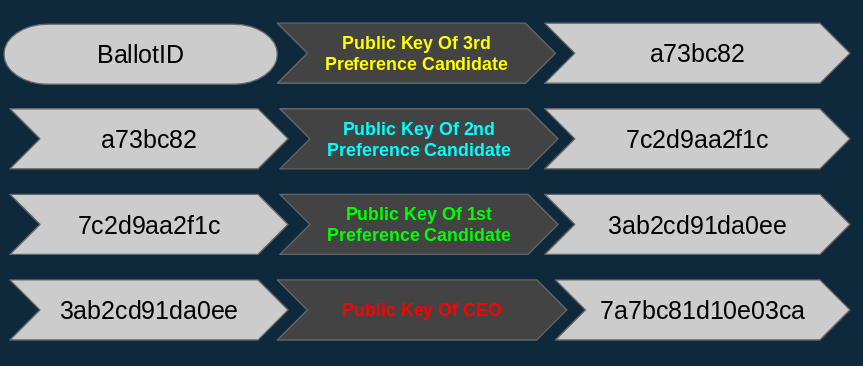
\includegraphics[width=\linewidth]{encryption.png}
        \caption{Encryption process}
        \label{fig:boat1}
    \end{figure}
    \tab This is the final vote that is sent to the server.\\
    \tab Also, the Ballot ID is encrypted symmetrically using the password of the voter and is sent to the server along with the vote.\\

\subsection{Calculation and Declaration of Results}
    \tab The CEO logs into his account and clicks on a button to stop voting. No votes will be accepted by the server after this.\\
    \tab The candidates then log into their accounts, decrypt their private keys using their passwords, and send their unencrypted private keys to the server.\\
    \tab The CEO now has access to his own private key, and the unencrypted private keys of all the candidates. He fetches all the votes from the server and performs the following operations on them :
    \begin{itemize}
        \item He decrypts each vote them from his own private key. This gives him an object that he needs to further decrypt.
        \item He then tries to decrypt it using the private keys of all the candidates, one by one. Whichever candidate's private key successfully decrypts the vote, is on the 1st preference in that vote. The decryption results in a new object.
        \item Again, the CEO tries to decrypt it using the private keys of all the candidates, one by one. Whichever candidate's key successfully decrypts this object, is on the 2nd preference in that vote.
        \item The same procedure is repeated to get the 3rd preference in that vote. The final decryption gives him the Ballot ID that was used to cast that vote.
        \item This Ballot ID is published with the 1st, 2nd and 3rd preference candidates contained in the vote.
    \end{itemize}
    \tab Finally, the total 1st, 2nd and 3rd preference votes for each candidate are counted, sorted and published. This completes the election process.

\section{Answers to Frequently Raised Security Concerns}
    \tab Any system claiming to be secure always raises some questions. Here are a few remarks about some of the frequently raised concerns :
    \begin{itemize}
        \item \textit{How does the system ensure that the votes are anonymous?}\\
              \tab A vote is not bound to any voter, but to a Ballot ID. This Ballot ID is stored in the database encrypted by the voter's password. Thus, not even the System Admin can find out which vote corresponds to which voter.
        \item \textit{How does the system ensure that the System Admin does not modify any voter's vote?}\\
              \tab Each voter can log in and access the Ballot ID bound to his vote. He can then check the preferences against this Ballot ID in the list published by the CEO. The preferences mentioned there must match the preferences that the voter had filled while voting.
        \item \textit{How does the system ensure that the System Admin does not add ghost votes or delete someone's vote?}\\
              \tab The list of all the voters who voted in the elections is published. The number of voters must equal the number of votes counted. Also, the voters can verify that their names are on the list and the non-voters can verify that their votes are not on the list.
    \end {itemize}

\section{Unsolved Security Concerns}
    \tab The system is claimed to be \textit{cryptographically secure}. However, there are some security issues inherent in the idea of online elections.
    \tab One issue is the regarding the independence of choice of a voter's preferences. Since the voters have the comfort of voting from their own devices from any location, they can be forced to vote for a candidate by his supporters even if they don't want to vote for him. The main problem here is that \textit{a voter's location may not provide the safety of a polling booth.}\\
    \tab Another issue is regarding the anonymity of votes. If the system can prove to the voter that his vote was counted correctly, then any candidate can demand a voter to prove that the voter voted for him. This is again a social issue. This can be prevented by not declaring the Ballot IDs during the declaration of results. But in that case the voter will have to trust the System Admin.\\
    \tab Another issue that props up is that since the System Admin has access to the database at all times, he can run a script at the server that queries the database for all the voters who have voted at that time, and also for the list of all the encrypted votes. Any new addition to the list of voters who have voted can be mapped to any new vote in the database. This vote, although encrypted now, will be unencrypted later and then the System Admin will know the preferences of all the voters. This is a flaw in the system and has been solved, \textit{albeit in a hacky way}, by delaying the addition of votes into the database. So when a new vote is received by the server, it is stored in the program's memory for a random period of time (the maximum limit of which is set during initialization), while the voter is immediately marked as voted. After the random time period is over, the vote is inserted into the database. Thus, the System Admin cannot create a mapping.\footnote[2]{One can claim that the System Admin can still hack into the program's memory and access the vote. However, this step certainly makes it extremely difficult for the System Admin to create such a mapping. Nevertheless, the concern is valid and hence this issue is put in this section.}

\section{Implementation}
    \tab The source code of the application is available on GitHub at \href{https://github.com/dryairship/online-election-manager}{https://github.com/dryairship/online-election-manager}\\
    \tab The backend is implemented in \href{https://golang.org/}{\textit{Golang}}, using the \href{https://github.com/gin-gonic/gin}{\textit{gin}} web framework.\\
    \tab \href{https://jquery.com/}{\textit{jQuery}} is used at the frontend to communicate with the API of the backend.\\
    \tab \href{https://www.mongodb.com/}{\textit{MongoDB}} is used for data storage.\\
    \tab Stanford University's \href{https://github.com/bitwiseshiftleft/sjcl}{\textit{sjcl}} is used for encryption.\\

\section{Results}
\tab The application was aimed at solving the problem of holding elections online. Although the system is claimed to be cryptographically secure, we still fall short of realizing an ideal model because of lack of security in the social domain. Improving the model to make it socially secure is an option for future work in this field.
\begin{thebibliography}{99}
\bibitem[1]{PuppyLove}
Saksham Sharma\\
\newblock \href{https://github.com/pclubiitk/puppy-love/raw/master/frontend/src/assets/report.pdf}{\textbf{Puppy Love} : \textit{Cryptographically secure anonymous couple matching}}
\end{thebibliography}

\end{document}
